% This is a complete LaTeX document for a Use Case Specification.
%
% Revision 6 (Full Document):
% 1. Updated author and date as requested.
% 2. Corrected 'Actors' section (Internal components removed).
% 3. Renamed external systems as 'Secondary Actors' (standard).
% 4. Added \midrule in table for readability.
% 5. Added \newpage before each Use Case.
% 6. Uses <description> list for UC metadata.
% 7. Uses high-level, non-technical language.

\documentclass{article}
\hbadness=10000                       % Suppress Warnings (Horizontal)
\vbadness=10000                       % Suppress Warnings (Vertical)

% -------------------------------------------------------------------
% \ PACKAGES
% -------------------------------------------------------------------

% Encoding
\usepackage[utf8]{inputenc} % Handle UTF-8 input
\usepackage[T1]{fontenc}    % Use modern font encoding
\usepackage{lmodern}        % Latin Modern (avoids EC/knappen Metafont "undefined x coordinate" font warnings)
\usepackage[english]{babel} % Set English as the primary language

% Page Layout
\usepackage[margin=1in]{geometry} % Set 1-inch margins (standard)
\usepackage{parskip}            % Use spacing between paragraphs, not indents


% Graphics and Diagrams
\usepackage{graphicx}
\usepackage{tikz}
\usetikzlibrary{shapes,arrows,positioning,fit,backgrounds,shadows,arrows.meta,calc,babel}

% Tables
\usepackage{tabularx}           % For tables that fit text width
\usepackage{booktabs}           % For professional-looking table rules (\toprule, etc.)

% Headers & Footers
\usepackage{fancyhdr}           % For custom headers and footers
\pagestyle{fancy}
\fancyhf{}                     % Clear all header and footer fields
\fancyhead[L]{System Design Documentation \textbar \ 24/7 Legal Intake Website}
\fancyfoot[C]{\thepage}
\renewcommand{\headrulewidth}{0.4pt} % Add a rule under the header

% Hyperlinks
\usepackage{hyperref}           % For clickable links (e.g., mailto:)
% \hypersetup{
%   colorlinks=true,
%   linkcolor=blue,
%   urlcolor=blue,
%   pdftitle={Use Case Specification: JS Law Group Website},
%   pdfauthor={Jaehoon Song}
% }

% -------------------------------------------------------------------
% \ TITLE INFORMATION
% -------------------------------------------------------------------
\title{System Design Documentation \\ \vspace*{20pt} \large JS Law Group \\ \vspace*{20pt} 24/7 Legal Rescue Website}
\author{Jaehoon Song}
\date{\today}


% -------------------------------------------------------------------
% \ DOCUMENT START
% -------------------------------------------------------------------
\begin{document}

\maketitle

\tableofcontents


% Behavioral Diagrams

% | Diagram          | Purpose           |
% | ---------------- | ----------------- |
% | Use case diagram | user interactions |
% | Activity diagram | workflows         |
% | State diagram    | state changes     |

% **Interaction Diagrams (subset of Behavioral)

% | Diagram               | Purpose              |
% | --------------------- | -------------------- |
% | Sequence diagram      | message order        |
% | Communication diagram | object communication |

% Structural Diagrams

% | Diagram            | Purpose                                      |
% | ------------------ | -------------------------------------------- |
% | Class diagram      | classes and relationships                    |
% | Object diagram     | snapshot of objects                          |
% | Component diagram  | software components                          |
% | Deployment diagram | hardware (you didn't list, but belongs here) |
% | Package diagram    | grouping (not listed but structural)         |





\newpage
% -------------------------------------------------------------------
% \ SECTION 1: REQUIREMENTS: FUNCTIONAL AND NON-FUNCTIONAL
% -------------------------------------------------------------------
\section{Requirements: Functional and Non-Functional}\label{sec:requirements}
This document captures the baseline functional and non-functional 
requirements for the JS Law Group marketing website. It serves as the 
authoritative guide for all development, quality assurance (QA), 
and future enhancement work.
\subsection{Scope}
The scope of this system covers the public-facing, multilingual web 
application for clients in emergency situations. The website contains 
minimal contact and law firm information (e.g., practice area summary, 
address, social links, emergency call, wizard) so users can quickly 
request help. Content presentation focuses on practice areas and the 
client contact intake workflow via the Auto Accident Wizard. The 
application is implemented as a Python Flask backend with server-side 
form processing, validation (Flask-WTF), and email dispatch (GmailProxy).

Payment processing, user authentication, and internal case management systems are intentionally out of scope for this project.


% -------------------------------------------------------------------
% \ FUNCTIONAL REQUIREMENTS
% -------------------------------------------------------------------
\subsection{Functional Requirements}

\subsubsection{Site Shell and Navigation}
\begin{enumerate}
  \item \textbf{FR-01: Consistent Shell.} The system \textbf{shall} display a consistent navigation header and footer across all sections of the site.
  \item \textbf{FR-02: Fixed Navigation.} The main navigation menu \textbf{shall} remain fixed at the top of the screen. It \textbf{shall} provide links to all main content sections and \textbf{shall} collapse into a mobile-friendly menu icon on small screens.
  \item \label{fr:03} \textbf{FR-03: Landing Hero.} The main landing section \textbf{shall} display a translated headline, a subtitle, and summary cards for the main practice areas (Personal Injury, Criminal Defense, Family Law). The section \textbf{shall} also provide three separate, independent elements: (1) a call-to-action button, (2) a main website button or link, and (3) the Accident Wizard, which \textbf{shall} be present in the hero section. These three \textbf{shall} not depend on each other.
\end{enumerate}

\subsubsection{Localized Content Delivery}
\begin{enumerate}
  \item \textbf{FR-04: Locale Management.} The system \textbf{shall} manage translations using JSON-based locale files (e.g., \texttt{en-US.json}, \texttt{ko-KR.json}, \texttt{ja-JP.json}, \texttt{es-US.json}) in a central \texttt{static/locales/} (or equivalent) directory. English \textbf{shall} be the default fallback language.
  \item \textbf{FR-05: Runtime Switching.} Language options \textbf{shall} be provided on the Floating Action Button (FAB). Selecting a language \textbf{shall} immediately translate all text on the page via the i18n system and \textbf{shall} persist the user's choice (e.g., in LocalStorage) for future visits.
  \item \textbf{FR-06: Translatable Content.} All visitor-facing text \textbf{shall} be sourced from the central translation files and \textbf{shall} be wired for translation (e.g., via \texttt{data-i18n} or equivalent). This includes articles, labels, buttons, and form fields.
  \item \textbf{FR-07: State Refresh.} The system \textbf{shall} refresh its state when the browser tab regains focus, ensuring the most recent content and language setting are displayed.
  \item \label{fr:08} \textbf{FR-08: Practice Detail Sections.} The site \textbf{shall} feature dedicated sections for Personal Injury and Criminal Defense, showing relevant imagery and bulleted lists of services. Content is kept minimal for emergency-focused users.
\end{enumerate}

\subsubsection{Engagement and Intake}
\begin{enumerate}
  \item \textbf{FR-09: Independent Engagement Controls.} The system \textbf{shall} provide a call-to-action button, a main website button (or link) to the main firm website, and the Accident Wizard (in the hero section) as separate, independent controls. None of these \textbf{shall} depend on the others; each \textbf{shall} function on its own.
  \item \label{fr:10} \textbf{FR-10: Accident Wizard Form.} The Auto Accident Wizard \textbf{shall} be the sole form for submitting case inquiries. It \textbf{shall} collect accident type, details (e.g., ZIP code, medical treatment, police report status), and contact information (name, email, phone) in a multi-step flow. Form handling \textbf{shall} use Flask-WTF/WTForms with CSRF protection and server-side validation.
  \item \textbf{FR-11: Backend Email Dispatch.} Upon wizard submission, the system \textbf{shall} validate inputs and dispatch a structured inquiry email to the firm via the configured Gmail SMTP service (using \texttt{GmailProxy}), with attachments (e.g., JSON, CSV, HTML) as implemented. Submissions \textbf{shall} be stored on the server in a controlled \texttt{submissions/} directory for intake and audit purposes. The system \textbf{shall} send a phone/SMS follow-up to the client via the Twilio API right after submission (incident follow-up). The system \textbf{shall} register submitters (and optionally relatives or close contacts) with the Mailchimp API for the law firm's marketing and advertise email campaigns (see \ref{uc:07}).
  \item \textbf{FR-12: Floating Action Button.} A ``Floating Action Button'' (FAB) \textbf{shall} be visible on mobile for switching languages (e.g., opening the language selector).
  \item \label{fr:13} \textbf{FR-13: Contact Section.} The contact section \textbf{shall} display the firm's address and hyperlinks to the firm's official Facebook and Instagram only. It \textbf{shall} not include a map, phone links, or email links.
  \item \textbf{FR-14: Social Links.} The footer \textbf{shall} provide links to the firm's verified social media profiles (e.g., Facebook, Instagram) and static policy pages.
\end{enumerate}

\subsubsection{Backend Logic (Python Flask)}
\begin{enumerate}
  \item \textbf{FR-15: Routing.} The application \textbf{shall} use Flask to route URL requests to appropriate view functions (e.g., \texttt{/}, \texttt{/motor-vehicle-accident}).
  \item \textbf{FR-16: Form Validation.} The system \textbf{shall} use \texttt{Flask-WTF} and \texttt{WTForms} to validate all user inputs server-side, ensuring required fields and data formats (e.g., email, phone) are correct.
  \item \textbf{FR-17: CSRF Protection.} All forms \textbf{shall} include a CSRF token to prevent Cross-Site Request Forgery attacks.
  \item \textbf{FR-18: OS Detection.} The \texttt{main.py} wrapper \textbf{shall} automatically detect the operating system:
  \begin{itemize}
    \item \textbf{Windows:} Launch \texttt{Waitress} WSGI server.
    \item \textbf{Linux/macOS:} Launch \texttt{Gunicorn} WSGI server.
  \end{itemize}
\end{enumerate}

\subsubsection{Email Automation Service}
\begin{enumerate}
  \item \textbf{FR-19: SMTP Integration.} The \texttt{GmailProxy} service \textbf{shall} authenticate with a Gmail SMTP server using secure app passwords.
  \item \textbf{FR-20: Data Persistence.} Upon form submission, the system \textbf{shall} save the data locally in \texttt{submissions/} as:
  \begin{itemize}
    \item \texttt{.json} (raw data object)
    \item \texttt{.csv} (comma-separated values)
    \item \texttt{.html} (formatted body)
  \end{itemize}
  \item \textbf{FR-21: Attachment Handling.} The system \textbf{shall} attach the generated JSON and CSV files to the notification email sent to the firm.
\end{enumerate}

\subsubsection{Frontend \& Internationalization (i18n)}
\begin{enumerate}
  \item \textbf{FR-22: Bilingual Implementation.} The system \textbf{shall} support dynamic switching between English (en-US), Korean (ko-KR), Japanese (ja-JP), and Spanish (es-US) using a custom JSON-based i18n module.
  \item \textbf{FR-23: Responsive Implementation.} The UI \textbf{shall} utilise Bootstrap 5 to ensure full responsiveness across mobile, tablet, and desktop devices.
  \item \textbf{FR-24: Debug Mode.} The system \textbf{shall} provide a visual debug mode to highlight translated elements for developers.
\end{enumerate}

% -------------------------------------------------------------------
% \ NON-FUNCTIONAL REQUIREMENTS
% -------------------------------------------------------------------
\subsection{Non-Functional Requirements}
\begin{enumerate}
  \item \textbf{NFR-01: Responsive Layout.} The website layout \textbf{shall} be fully responsive using a mobile-first approach, adapting cleanly to desktop, tablet, and mobile screen sizes without horizontal scrolling.
  \item \textbf{NFR-02: Accessibility.} The website \textbf{shall} adhere to Web Content Accessibility Guidelines (WCAG) AA standards. This includes use of semantic HTML5, alt text for images, and full keyboard navigation support.
  \item \textbf{NFR-03: Performance.} The website \textbf{shall} load quickly. External resources (fonts, icons) \textbf{shall} be loaded from a Content Delivery Network (CDN). The Largest Contentful Paint (LCP) \textbf{shall} be under 2.5 seconds on a standard broadband connection. Frontend \textbf{shall} use a modular JavaScript architecture and optimized asset delivery as documented in the project.
  \item \textbf{NFR-04: Privacy and Security.} Personally Identifiable Information (PII) \textbf{shall} only be collected via the Accident Wizard form and \textbf{shall} be handled in accordance with the firm's privacy policy. The system \textbf{shall} store submissions only in the controlled \texttt{submissions/} directory and transmit them to the firm via Gmail SMTP. The system \textbf{shall} only use local browser storage for language preferences. A privacy statement \textbf{shall} be included in the footer.
  \item \textbf{NFR-05: Localization Quality.} When new content is added, corresponding translations \textbf{shall} be added for all supported languages to avoid displaying fallback (English) text.
  \item \textbf{NFR-06: Maintainability.} All new code \textbf{shall} be modular, separated from content (e.g., translations in JSON, templates in \texttt{templates/}, styles in \texttt{static/}), and well-documented to ensure future maintainability.
  \item \textbf{NFR-07: Availability and Hosting.} The system \textbf{shall} be implemented as a Python Flask application. It \textbf{shall} be hostable using a production WSGI server: Waitress on Windows and Gunicorn on Linux/Mac. The application \textbf{shall} support optional bundling as a standalone executable (e.g., via PyInstaller) for target platforms.
  \item \textbf{NFR-08: Browser Support.} The system \textbf{shall} be fully functional on the two most recent versions of Chrome, Safari, Edge, and Firefox on both desktop and mobile platforms.
\end{enumerate}

% -------------------------------------------------------------------
% \ DEPENDENCIES AND CONSTRAINTS
% -------------------------------------------------------------------
\subsection{Dependencies and Constraints}
\begin{itemize}
  \item The system \textbf{is constrained} to use the Bootstrap 5 framework for layout and responsive behavior.
  \item The system \textbf{is constrained} to use the Font Awesome 6 icon library for UI icons.
  \item The system \textbf{is dependent} on the Google Fonts service for typography (e.g., Inter, Noto Sans KR as documented in the project).
  \item The system \textbf{is dependent} on Python Flask, Flask-WTF/WTForms for form handling and CSRF protection, and a production WSGI server (Waitress or Gunicorn) for deployment.
  \item The contact workflow \textbf{is dependent} on the backend having valid Gmail SMTP credentials (for \texttt{GmailProxy}) and outbound network access to the Gmail service.
  \item The system \textbf{is dependent} on the user's browser supporting LocalStorage for persisting language preferences.
  \item The system \textbf{is dependent} on the Twilio API for sending a phone/SMS follow-up to the client right after wizard submission (incident follow-up).
  \item The system \textbf{is dependent} on the Mailchimp API to register inquiry submitters (and optionally relatives or close contacts) for the law firm's marketing and advertise email campaigns.
\end{itemize}













\newpage
% -------------------------------------------------------------------
% \ STAKEHOLDERS
% -------------------------------------------------------------------
\section{Behavioral Specification: Use Case Analysis}\label{sec:usecases}
This section describes the behavioral specification of the 24/7 Legal Intake Website 
through use case analysis. It identifies stakeholders and actors, presents a 
use case diagram, and provides fully dressed use case descriptions for development and QA.\footnote{
  \textbf{Activity diagrams} and \textbf{communication diagrams} have been omitted, 
  as the system does not have the complexity that would warrant those diagrams.
}

\subsection{Stakeholders}

\begin{tabularx}{\textwidth}{@{} p{3.2cm} X @{}}
\toprule
\textbf{Stakeholder} & \textbf{Goals and Concerns} \\
\midrule
Prospective Clients & Need fast access to practice area information, bilingual copy, and an immediate way to request help (emergency call or wizard) without sharing payment or sensitive data online. \\
\midrule % Added for readability
Family or Community Referrals & Want minimal firm information (office address, social links) on behalf of someone in need. \\
\midrule % Added for readability
Attorneys and Intake Staff & Need complete, well-formatted inquiries routed to the firm's intake email so follow-ups can be triaged quickly. \\
\midrule % Added for readability
Marketing/Admin Team & Owns site content, translations, imagery, and compliance statements; cares about maintainable assets and accurate brand voice. \\
\midrule % Added for readability
Technology Operations & Maintains the website hosting and ensures all website dependencies remain reachable and secure. \\
\bottomrule
\end{tabularx}

% -------------------------------------------------------------------
% \ ACTORS
% -------------------------------------------------------------------
\subsection{Actors}

\subsubsection{Primary Actors}
\begin{itemize}
  \item \textbf{Prospective Client (English).} A person seeking legal representation who speaks English.
  \item \textbf{Prospective Client (Bilingual).} A person seeking legal representation who prefers to read in Korean, Japanese, or Spanish.
  \item \textbf{Referral or Family Member.} A person collecting information (e.g., address, social links) on behalf of someone else.
\end{itemize}

\subsubsection{Secondary Actors (External Systems and APIs)}
\begin{itemize}
  \item \textbf{Third-Party Content Services.} External hosts that the system relies on to provide fonts, icons, and other design assets.
  \item \textbf{Gmail SMTP Service.} The email transport service used by the backend to dispatch inquiry notifications and wizard submissions.
  \item \textbf{Twilio API.} Messaging service used by the backend to send a phone/SMS follow-up to the client right after they submit the Accident Wizard form (incident-related follow-up).
  \item \textbf{Mailchimp Marketing API.} External service used to register inquiry submitters (and optionally their relatives or close contacts) so the law firm can send them marketing and advertise emails for follow-up and ongoing connection.
\end{itemize}




% -------------------------------------------------------------------
% \ USE CASE DIAGRAM AND CATALOG
% -------------------------------------------------------------------
\newpage
\subsection{Use Case Diagram}\label{ss:usecasediag}
Figure~\ref{fig:usecase_diag} shows actors and use cases for the 24/7 Legal Intake Website.

\begin{figure}[htbp]
  \centering
  \begin{tikzpicture}[
    % Standard UML Actor (Stickman)
    actor/.style={
      male, % requires \usetikzlibrary{shapes.multipart} or custom stickman
      draw, 
      thick, 
      minimum black line/.style={draw=black, thick},
      inner sep=0pt,
      minimum width=0.8cm
    },
    % UML Use Case (Ellipse)
    usecase/.style={
      ellipse, 
      draw, 
      minimum width=3cm, 
      minimum height=1cm, 
      align=center, 
      font=\small
    },
    % System Boundary (fit around use cases, no fixed size)
    system/.style={
      rectangle, draw, thick,
      inner sep=14pt
    },
    % Secondary actor box
    ext/.style={
      draw, rectangle, thick,
      minimum width=1.8cm, minimum height=0.65cm,
      font=\small
    }
  ]
  
  % Custom Stickman Definition for standard UML
  \tikzset{
    stickman/.style={
      draw, circle, inner sep=0pt, minimum size=0.5cm,
      append after command={
        node[below=0.1cm of \tikzlastnode.south, inner sep=0pt] (\tikzlastnode-body) {}
        (\tikzlastnode.south) edge (\tikzlastnode.south |- [yshift=-0.6cm]\tikzlastnode.south)
        ([yshift=-0.2cm]\tikzlastnode.south) edge ++(-0.3cm,-0.2cm)
        ([yshift=-0.2cm]\tikzlastnode.south) edge ++(0.3cm,-0.2cm)
        ([yshift=-0.6cm]\tikzlastnode.south) edge ++(-0.25cm,-0.4cm)
        ([yshift=-0.6cm]\tikzlastnode.south) edge ++(0.25cm,-0.4cm)
      }
    }
  }
  
  % Use Cases (Vertically Stacked)
  \node[usecase] (uc1) at (3.5,  0.0) {Select Site Language};
  \node[usecase] (uc2) at (3.5, -1.2) {Research Practice Areas};
  \node[usecase] (uc3) at (3.5, -2.4) {Use Emergency Call};
  \node[usecase] (uc4) at (3.5, -3.6) {Open Main Website};
  \node[usecase] (uc5) at (3.5, -4.8) {View Address \& Social};
  \node[usecase] (uc6) at (3.5, -6.0) {Submit Accident Wizard};
  \node[usecase] (uc7) at (3.5, -7.2) {Register for Marketing};
  
  % System Boundary: fit tightly around use cases
  \node[system, fit=(uc1) (uc7), label={[anchor=north west, font=\bfseries]north west:24/7 Legal Intake Website}] (boundary) {};
  
  % Primary Actors (Left)
  \node[label=below:{\small Prospective Client}] (client) at (-1.5, -1.5) {
    \begin{tikzpicture}[scale=0.4]
      \draw (0,0) circle (0.3); \draw (0,-0.3) -- (0,-1.2);
      \draw (-0.5,-0.6) -- (0.5,-0.6); \draw (0,-1.2) -- (-0.4,-1.8); \draw (0,-1.2) -- (0.4,-1.8);
    \end{tikzpicture}
  };
  
  \node[label=below:{\small Referral / Family}] (referral) at (-1.5, -4.8) {
    
\begin{tikzpicture}[scale=0.4]
      \draw (0,0) circle (0.3); \draw (0,-0.3) -- (0,-1.2);
      \draw (-0.5,-0.6) -- (0.5,-0.6); \draw (0,-1.2) -- (-0.4,-1.8); \draw (0,-1.2) -- (0.4,-1.8);
    \end{tikzpicture}
  };
  
  % Secondary Actors (Right)
  \node[ext, right=2.8cm of uc4.east] (admin) {Firm Admin};
  \node[ext, below=0.56cm of admin] (gmail) {Gmail SMTP};
  \node[ext, below=0.56cm of gmail] (twilio) {Twilio API};
  \node[ext, right=2.4cm of uc7.east] (mailchimp) {Mailchimp API};
  
  % Associations
  \draw (client) -- (uc1);
  \draw (client) -- (uc2);
  \draw (client) -- (uc3);
  \draw (client) -- (uc4);
  \draw (client) -- (uc5);
  \draw (client) -- (uc6);
  
  \draw (referral) -- (uc5);
  
  \draw (admin) -- (uc6);
  \draw (admin) -- (uc7);
  \draw (gmail) -- (uc6);
  \draw (twilio) -- (uc6);
  \draw (mailchimp) -- (uc7);
  
  \end{tikzpicture}
  \caption{UML Use Case Diagram - actors and use cases for the 24/7 Legal Intake Website}
  \label{fig:usecase_diag}
\end{figure}

\subsection{Use Cases (Fully Dressed)}
\subsubsection{UC-01: Select a Site Language}\label{uc:01}
\begin{description}
  \item[Primary Actor:] Prospective client (bilingual)
  \item[Secondary Actors:] User's Browser
  \item[Goal:] View all copy in a preferred language to evaluate the firm comfortably.
  \item[User Story:] As a Korean-speaking client, I want to flip the site into Korean so I can confirm services and contact steps without translation mistakes.
  \item[Preconditions:] The website has fully loaded in the default language.
  \item[Trigger:] The visitor opens the FAB and clicks one of the language options.
\end{description}
\textbf{Main Scenario:}
\begin{enumerate}
  \item The actor activates the Floating Action Button (FAB) to open the language selector.
  \item The actor selects a locale option (e.g., ``Korean'' or ``Spanish'' or ``Japanese'').
  \item The system retrieves the corresponding text and updates every label, button, and article on the page.
  \item The system saves this language choice in the user's browser, so it is remembered on future visits.
\end{enumerate}
\textbf{Alternate Flows:}
\begin{itemize}
  \item If the translation file cannot be loaded (e.g., network disruption), the system logs an error, and the website remains in the previous language.
\end{itemize}
\textbf{Postconditions:} The chosen language persists for the session. All subsequent actions and popups are shown in the selected language.

\subsubsection{UC-02: Research Practice Areas}
\begin{description}
  \item[Primary Actor:] Prospective client (any language)
  \item[Secondary Actors:] Third-Party Content Services (for images)
  \item[Goal:] Understand whether JS Law Group covers the specific legal scenario at hand.
  \item[User Story:] As someone recovering from a collision, I want to skim the Personal Injury section and content to determine if the firm handles car and premises cases.
  \item[Preconditions:] The website is loaded.
  \item[Trigger:] The actor lands on the site or scrolls / clicks ``Practice Areas''.
\end{description}
\textbf{Main Scenario:}
\begin{enumerate}
  \item The actor glances at the main service cards to confirm the firm covers PI, Criminal Defense, and Family Law.
  \item The actor scrolls to the Personal Injury section, reviewing the translated bullet list of featured services and any minimal copy.
  \item If relevant, the actor repeats the process with the Criminal Defense section.
  \item The actor may use the emergency call or the Accident Wizard if ready to proceed.
\end{enumerate}
\textbf{Alternate Flows:}
\begin{itemize}
  \item On mobile, the actor may use the main menu to jump directly to practice sections or to the wizard.
\end{itemize}
\textbf{Postconditions:} The actor has enough information to decide whether to contact the firm (e.g., via emergency call or wizard).

\subsubsection{UC-03: Use Emergency Call Button}
\begin{description}
  \item[Primary Actor:] Prospective client ready to contact
  \item[Secondary Actors:] User's Phone/Voice Application
  \item[Goal:] Immediately place a phone call to the firm in an urgent situation.
  \item[User Story:] As a client in an emergency, I want one tap to call the firm so I can speak to someone right away.
  \item[Preconditions:] The emergency call button is visible on the screen (mobile or desktop).
  \item[Trigger:] The actor clicks or taps the emergency call button.
\end{description}
\textbf{Main Scenario:}
\begin{enumerate}
  \item The actor activates the emergency call button.
  \item The system invokes the device's dialer with the firm's phone number pre-filled.
  \item The actor confirms or places the call.
\end{enumerate}
\textbf{Alternate Flows:}
\begin{itemize}
  \item If the device cannot place calls (e.g., no telephony capability), the system shows the firm's phone number so it can be dialed from another device.
\end{itemize}
\textbf{Postconditions:} The actor is in a position to speak with the firm by phone, or has the number needed to do so.

\newpage
\subsubsection{UC-04: Open Main Firm Website}
\begin{description}
  \item[Primary Actor:] Prospective client wanting more background about the firm
  \item[Secondary Actors:] Web browser
  \item[Goal:] View the full JS Law Group website for deeper information (e.g., history, additional services).
  \item[User Story:] As a client researching the firm, I want a clear button that takes me to the main website so I can read more before deciding to call.
  \item[Preconditions:] The redirect button or link to the main website is visible.
  \item[Trigger:] The actor clicks the ``Visit Main Website'' button.
\end{description}
\textbf{Main Scenario:}
\begin{enumerate}
  \item The actor clicks the redirect button.
  \item The system opens the main JS Law Group website in the same tab or a new tab, as configured.
\end{enumerate}
\textbf{Alternate Flows:}
\begin{itemize}
  \item If the main website is temporarily unavailable, the system shows an error message or fallback contact information.
\end{itemize}
\textbf{Postconditions:} The actor can browse the main firm website for additional details about the practice.

\subsubsection{UC-05: View Address and Social Links}
\begin{description}
  \item[Primary Actor:] Referral / family member confirming logistics
  \item[Secondary Actors:] Web browser
  \item[Goal:] Obtain the office address and hyperlinks to the firm's official Facebook and Instagram.
  \item[User Story:] As a friend helping someone find the firm, I want to see the address and links to the firm's official social profiles so I can share them.
  \item[Preconditions:] The website is loaded.
  \item[Trigger:] The actor scrolls or navigates to the contact section.
\end{description}
\textbf{Main Scenario:}
\begin{enumerate}
  \item The actor scrolls to or navigates to the contact section.
  \item The actor reviews the firm's address (plain text).
  \item The actor uses the hyperlinks to open the firm's official Facebook and Instagram profiles.
\end{enumerate}
\textbf{Alternate Flows:}
\begin{itemize}
  \item If the contact section cannot be loaded correctly, the system still displays at least the address and social links in plain text.
\end{itemize}
\textbf{Postconditions:} The actor has the office address and can access the firm's official Facebook and Instagram pages.

\newpage
\subsubsection{UC-06: Submit Auto Accident Wizard}\label{uc:06}
\begin{description}
  \item[Primary Actor:] Prospective client.
  \item[Secondary Actors:] Email Service Provider (Gmail); Firm Administrator; Twilio API (phone/SMS incident follow-up).
  \item[Goal:] Complete a multi-step assessment to report a motor vehicle accident.
  \item[Preconditions:] The user is on the homepage; the Accident Wizard is present in the hero section and visible.
  \item[Trigger:] The user interacts with the ``Accident Wizard'' form.
\end{description}
\textbf{Main Scenario:}
\begin{enumerate}
  \item The user selects the accident type (``Car'' or ``Motorcycle'' or etc.) and provides accident details (ZIP code, medical treatment, police report status, and related fields).
  \item The user enters contact information (name, email, phone).
  \item The system validates all inputs (CSRF token, email format, and related fields).
  \item The system dispatches a structured email to the Firm Administrator via Gmail SMTP with the JSON/CSV attachments after processing the form via Flask-WTF.
  \item The system sends a phone/SMS follow-up to the client via the Twilio API (incident follow-up right after submission).
  \item The system displays a success confirmation to the user.
\end{enumerate}
\textbf{Postconditions:} An inquiry email with attachments is delivered to the Firm Administrator; the user sees a confirmation message; the client receives a phone/SMS follow-up via Twilio.
\subsubsection{UC-07: Register for Marketing Email (Mailchimp)}\label{uc:07}
\begin{description}
  \item[Primary Actor:] System (automated when inquiry data is available) or Firm Administrator.
  \item[Secondary Actors:] Mailchimp Marketing API.
  \item[Goal:] Register inquiry submitters (and optionally relatives or close contacts) in Mailchimp so the law firm can send them marketing and advertise emails (e.g., annual campaigns and follow-up).
  \item[Preconditions:] Wizard submission data has been received and stored (e.g., in \texttt{submissions/} or intake system).
  \item[Trigger:] New inquiry data is available for registration, or the Firm Administrator initiates sync to Mailchimp.
\end{description}
\textbf{Main Scenario:}
\begin{enumerate}
  \item The system (or administrator) sends the submitter's contact information (and optionally relatives or close contacts) to the Mailchimp API to add to the law firm's audience/list.
  \item Mailchimp registers the contact(s) for the firm's marketing and advertise email campaigns.
\end{enumerate}
\textbf{Postconditions:} The submitter (and optionally relatives or close contacts) is registered in Mailchimp; the law firm can send them marketing and annual advertise emails.


\newpage
\subsection{Sequence Diagrams}\label{ss:seqdiag}
The following sequence diagram captures the primary legal intake submission flow 
from the user's perspective through to backend persistence and notification. 
It shows the main participants---User, Browser, Flask App, File System, and Gmail SMTP---and 
the order of interactions: the user accesses the site and receives the wizard (GET \texttt{/}), 
fills the 10-step Auto Accident form, and submits (POST \texttt{/}); 
the server validates input (e.g.\ via WTForms), 
saves the submission as JSON/CSV/HTML under \texttt{submissions/}, and 
sends a notification email via Gmail SMTP before returning a success response to the browser. 
Figure~\ref{fig:seq_diag} illustrates this flow.
\begin{figure}[htbp]
  \centering
  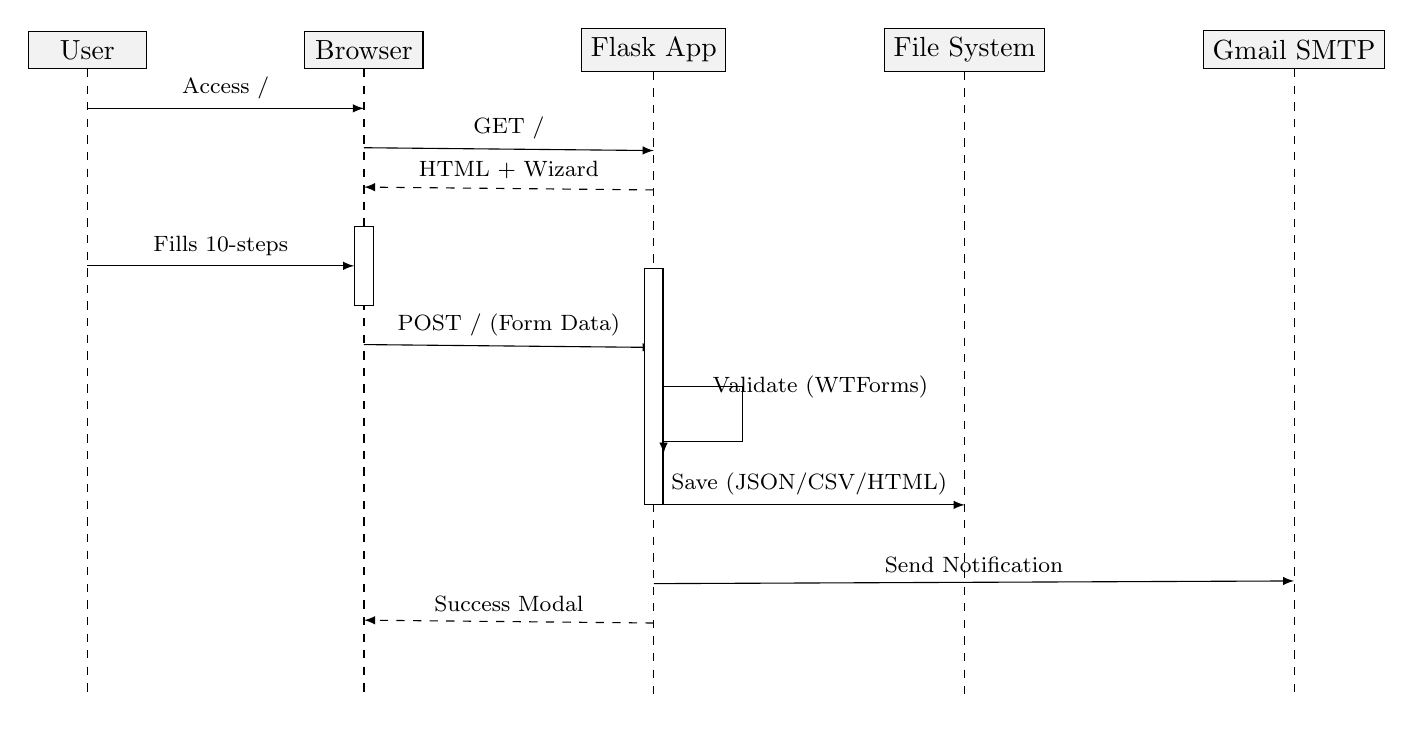
\begin{tikzpicture}[
    node distance=1.5cm,
    actor/.style={rectangle, draw, minimum width=1.5cm, fill=gray!10},
    lifeline/.style={draw, dashed},
    message/.style={-latex, font=\footnotesize},
    activation/.style={rectangle, draw, fill=white, minimum width=0.2cm}
  ]

  % Participants
  \node[actor] (user) {User};
  \node[actor, right=2cm of user] (browser) {Browser};
  \node[actor, right=2cm of browser] (flask) {Flask App};
  \node[actor, right=2cm of flask] (fs) {File System};
  \node[actor, right=2cm of fs] (gmail) {Gmail SMTP};

  % Lifelines
  \draw[lifeline] (user.south) -- +(0,-8);
  \draw[lifeline] (browser.south) -- +(0,-8);
  \draw[lifeline] (flask.south) -- +(0,-8);
  \draw[lifeline] (fs.south) -- +(0,-8);
  \draw[lifeline] (gmail.south) -- +(0,-8);

  % Interactions
  \draw[message] ($(user.south)+(0,-0.5)$) -- node[above] {Access /} ($(browser.south)+(0,-0.5)$);
  \draw[message] ($(browser.south)+(0,-1.0)$) -- node[above] {GET /} ($(flask.south)+(0,-1.0)$);
  \draw[message, dashed] ($(flask.south)+(0,-1.5)$) -- node[above] {HTML + Wizard} ($(browser.south)+(0,-1.5)$);

  \node[activation] at ($(browser.south)+(0,-2.5)$) [minimum height=1cm] (a1) {};
  \draw[message] ($(user.south)+(0,-2.5)$) -- node[above] {Fills 10-steps} (a1.west);

  \draw[message] ($(browser.south)+(0,-3.5)$) -- node[above] {POST / (Form Data)} ($(flask.south)+(0,-3.5)$);
  
  \node[activation] at ($(flask.south)+(0,-4.0)$) [minimum height=3cm] (a2) {};
  \draw[message] (a2.east) -- ++(1.0,0) node[right, midway] {Validate (WTForms)} -- ++(0,-0.7) -- ++(-1.0,0) -- ++(0,-0.15);
  
  \draw[message] ($(flask.south)+(0,-5.5)$) -- node[above] {Save (JSON/CSV/HTML)} ($(fs.south)+(0,-5.5)$);
  \draw[message] ($(flask.south)+(0,-6.5)$) -- node[above] {Send Notification} ($(gmail.south)+(0,-6.5)$);

  \draw[message, dashed] ($(flask.south)+(0,-7.0)$) -- node[above] {Success Modal} ($(browser.south)+(0,-7.0)$);

  \end{tikzpicture}
  \caption{UML Sequence Diagram - Legal Intake Submission Flow}
  \label{fig:seq_diag}
\end{figure}
\newpage
\subsection{State Diagram (UI Flow Diagram)}\label{ss:uiflow}
The diagram in Figure~\ref{fig:uiflow} illustrates the navigation paths and user interaction flow within the application.
\begin{figure}[htbp]
\centering
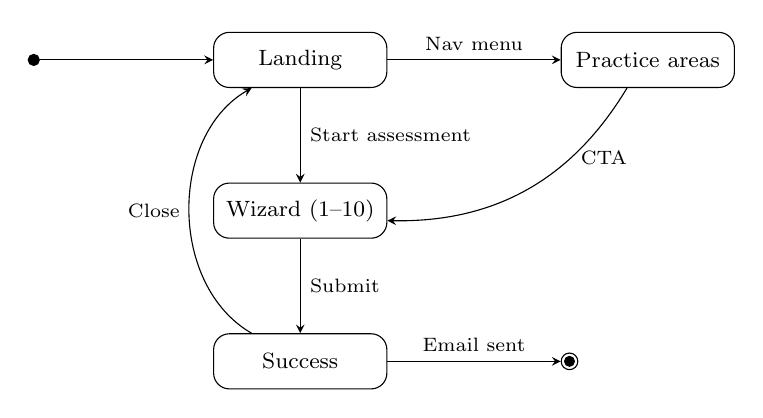
\begin{tikzpicture}[
    node distance=1.2cm and 2.2cm,
    >=stealth,
    % UML activity diagram styles
    initial/.style={circle, draw, fill=black, minimum size=4pt, inner sep=0},
    final/.style={circle, draw, minimum size=6pt, inner sep=0, path picture={\fill (path picture bounding box.center) circle (2pt);}},
    activity/.style={rectangle, draw, rounded corners=2mm, minimum width=2.2cm, minimum height=0.7cm, align=center, font=\footnotesize},
    flow/.style={->, draw}
  ]

  % Initial node
  \node[initial] (start) {};
  % Activities
  \node[activity, right=of start] (landing) {Landing};
  \node[activity, below=of landing] (wizard) {Wizard (1--10)};
  \node[activity, right=of landing] (practice) {Practice areas};
  \node[activity, below=of wizard] (success) {Success};
  \node[final, right=of success] (end) {};

  % Control flow
  \draw[flow] (start) -- (landing);
  \draw[flow] (landing) -- node[right, font=\scriptsize] {Start assessment} (wizard);
  \draw[flow] (landing) -- node[above, font=\scriptsize] {Nav menu} (practice);
  \draw[flow] (practice) to[bend left=30] node[right, font=\scriptsize, pos=0.3] {CTA} (wizard);
  \draw[flow] (wizard) -- node[right, font=\scriptsize] {Submit} (success);
  \draw[flow] (success) to[bend left=60] node[left, font=\scriptsize, pos=0.5] {Close} (landing);
  \draw[flow] (success) -- node[above, font=\scriptsize] {Email sent} (end);
\end{tikzpicture}
\caption{UML Activity Diagram - UI flow}
\label{fig:uiflow}
\end{figure}
\subsubsection{User Interface States}\label{ss:uistates}
\begin{itemize}
    \item \textbf{Landing State:} Users see the home page with the Auto Accident Wizard in 
    the hero section, plus call-to-action, main-website link, and practice-area summary 
    (FR-03 in \ref{sec:requirements}). The Floating Action Button (FAB) provides language 
    selection (\texttt{en-US}, \texttt{ko-KR}, \texttt{ja-JP}, \texttt{es-US}) with persistence 
    in LocalStorage (\ref{uc:01}).
    \item \textbf{Wizard State:} A single, progressive 10-step form 
    (accident type, ZIP, medical treatment, police report, prior attorney, accident date, 
    injury type, name, contact details, submit). It is the sole form for case inquiries 
    (FR-10 in \ref{sec:requirements}). Practice area pages link back to the wizard 
    (e.g.\ \texttt{\#wizard-container}) for inquiry CTAs.
    \item \textbf{Practice Area State:} Dedicated routes for \texttt{/motor-vehicle-accident} 
    and \texttt{/personal-injury}. The Personal Injury page includes a Criminal Defense section; 
    there is no separate Criminal Defense route. Content is minimal and i18n-enabled 
    (FR-08 in \ref{sec:requirements}).
    \item \textbf{Submission State:} After server-side validation (Flask-WTF, CSRF), 
    the user sees a success modal; data is written to \texttt{submissions/} (JSON, CSV, HTML) 
    and an email is sent via \texttt{GmailProxy}. Twilio follow-up and Mailchimp registration 
    are as specified in \ref{uc:06} and \ref{uc:07}.
\end{itemize}













\newpage
% -------------------------------------------------------------------
% \ SECTION 3: STRUCTURAL SPECIFICATION: SYSTEM ARCHITECTURE
% -------------------------------------------------------------------
\section{Structural Specification: System Architecture}\label{sec:architecture}
The JS Law Group's 24/7 Legal Intake Website application follows a Model-View-Controller (MVC) 
pattern adapted for Flask, deployed as a containerized application on cloud infrastructure.\footnote{
  \textbf{Class diagram}, \textbf{Object diagram}, and \textbf{Package diagram} have been omitted, 
  as the system does not have the complexity that would warrant those diagrams.
}
This section aligns with the functional and non-functional requirements (\ref{sec:requirements}), use cases (\ref{sec:usecases}), 
and the UI flow (\ref{fig:uiflow}).

\subsection{System Architecture Diagram}\label{ss:archdiag}

Figure~\ref{fig:arch_comp} shows the application components and their interfaces; Figure~\ref{fig:arch_deploy} shows the deployment topology on OCI.

\begin{figure}[htbp]
  \centering
  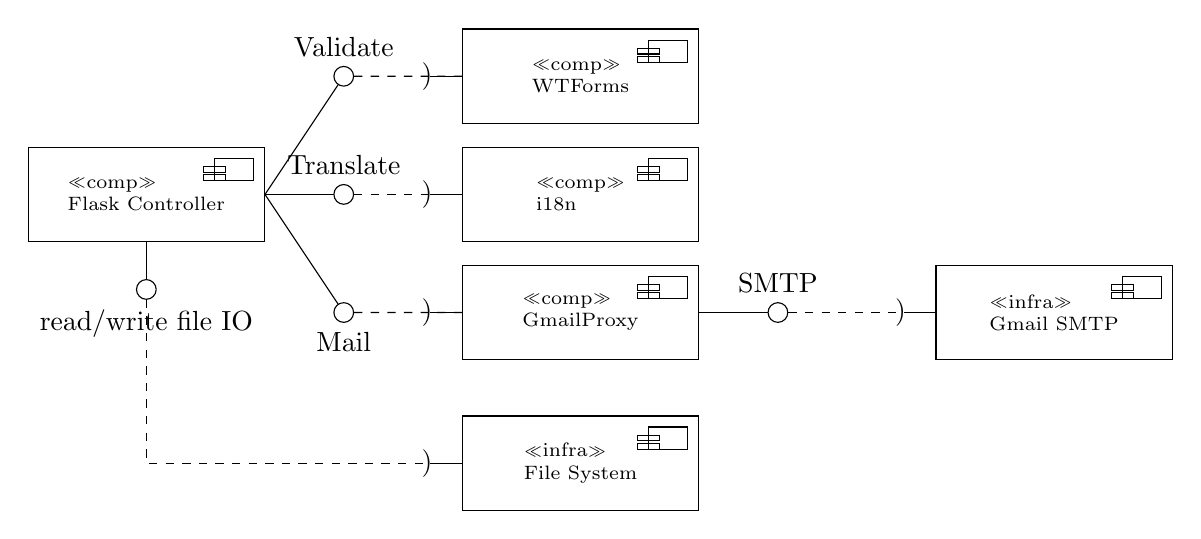
\begin{tikzpicture}[
    node distance=1.5cm and 2.5cm,
    component/.style={
      rectangle, draw, minimum width=3cm, minimum height=1.2cm,
      fill=white, align=left, font=\scriptsize,
      path picture={
        \draw ([xshift=-18pt, yshift=-12pt]path picture bounding box.north east)
          rectangle ([xshift=-4pt, yshift=-4pt]path picture bounding box.north east);
        \draw ([xshift=-22pt, yshift=-7pt]path picture bounding box.north east)
          rectangle ([xshift=-14pt, yshift=-9pt]path picture bounding box.north east);
        \draw ([xshift=-22pt, yshift=-10pt]path picture bounding box.north east)
          rectangle ([xshift=-14pt, yshift=-12pt]path picture bounding box.north east);
      }
    },
    dependency/.style={-latex, dashed},
    interface/.style={circle, draw, minimum size=2.5mm, inner sep=0pt, fill=white}
  ]
  \node[component] (flask) {\guillemotleft comp\guillemotright \\ Flask Controller};
  \node[component, right=of flask, yshift=1.5cm] (wtforms) {\guillemotleft comp\guillemotright \\ WTForms};
  \node[component, right=of flask] (i18n) {\guillemotleft comp\guillemotright \\ i18n};
  \node[component, right=of flask, yshift=-1.5cm] (gmail) {\guillemotleft comp\guillemotright \\ GmailProxy};
  \node[component, right=3cm of gmail] (smtp) {\guillemotleft infra\guillemotright \\ Gmail SMTP};
  \node[component, below=1cm of gmail, yshift=0.3cm] (fs) {\guillemotleft infra\guillemotright \\ File System};
  \draw (flask.east) -- ++(1.00,1.50) node[interface, label=above:Validate] (valid_ball) {};
  \draw (wtforms.west) -- ++(-0.4,0) node[anchor=east, xshift=0.15cm] {)};
  \draw[dashed] (valid_ball.east) -- (wtforms.west);
  \draw (flask.east) -- ++(1.00,0.00) node[interface, label=above:Translate] (lang_ball) {};
  \draw (i18n.west) -- ++(-0.4,0) node[anchor=east, xshift=0.15cm] {)};
  \draw[dashed] (lang_ball.east) -- (i18n.west);
  \draw (flask.east) -- ++(1.00,-1.50) node[interface, label=below:Mail] (mail_ball) {};
  \draw (gmail.west) -- ++(-0.4,0) node[anchor=east, xshift=0.15cm] {)};
  \draw[dashed] (mail_ball.east) -- (gmail.west);
  \draw (gmail.east) -- ++(1.0,0) node[interface, label=above:SMTP] (ball) {};
  \draw (smtp.west) -- ++(-0.4,0) node[anchor=east, xshift=0.15cm] {)};
  \draw[dashed] (ball.east) -- (smtp.west);
  \draw (flask.south) -- ++(0,-0.6) node[interface, label=below:read/write file IO] (io_ball) {};
  \draw (fs.west) -- ++(-0.4,0) node[anchor=east, xshift=0.15cm] {)};
  \draw[dashed] (io_ball.south) |- (fs.west);
  \end{tikzpicture}
  \caption{UML Component Diagram - application modules and external interfaces}
  \label{fig:arch_comp}
\end{figure}

\begin{figure}[htbp]
  \centering
  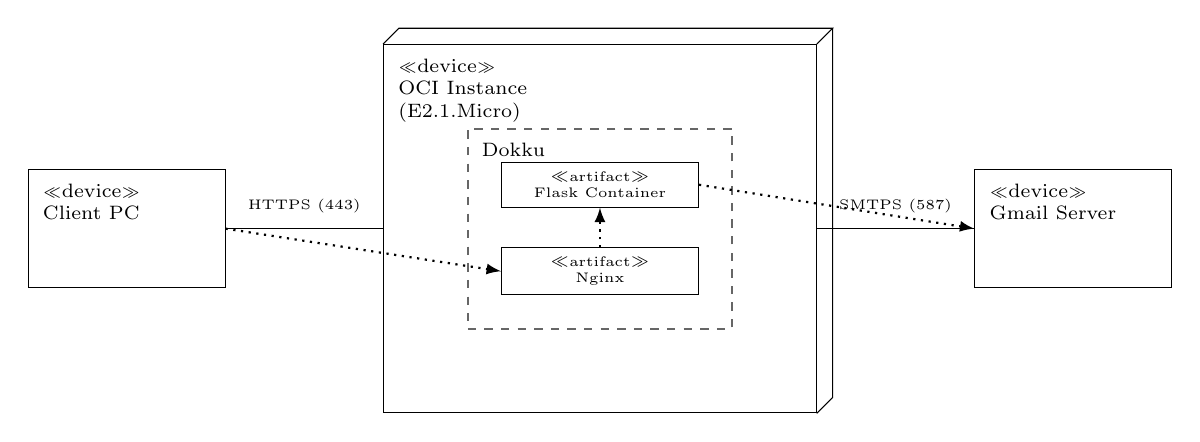
\begin{tikzpicture}[
    node distance=1.5cm,
    uml_node/.style={
      rectangle, draw,
      minimum width=2.5cm, minimum height=1.5cm,
      label={[anchor=north west, align=left, font=\scriptsize, xshift=2pt, yshift=-2pt]north west:{#1}}
    },
    group/.style={
      rectangle, draw, dashed, thick, draw=black!60,
      fill=none,
      label={[anchor=north west, align=left, font=\scriptsize, xshift=2pt, yshift=-2pt]north west:{#1}}
    },
    artifact/.style={
      rectangle, draw, fill=white,
      minimum width=2.5cm, font=\tiny, align=center
    },
    link/.style={draw, thin}
  ]
  \node[artifact] (flask) {\guillemotleft artifact\guillemotright \\ Flask Container};
  \node[artifact, below=0.5cm of flask] (nginx) {\guillemotleft artifact\guillemotright \\ Nginx};
  \node[group={Dokku}, inner sep=12pt, fit=(flask) (nginx)] (dokku) {};
  \node[uml_node={\guillemotleft device\guillemotright \\ OCI Instance \\ (E2.1.Micro)}, inner sep=30pt, fit=(dokku)] (oci) {};
  \node[uml_node={\guillemotleft device\guillemotright \\ Client PC}, left=2cm of oci.west] (client) {};
  \node[uml_node={\guillemotleft device\guillemotright \\ Gmail Server}, right=2cm of oci.east] (smtp) {};
  \draw[link] (client.east) -- node[above, font=\tiny, yshift=2pt] {HTTPS (443)} (oci.west);
  \draw[link] (oci.east) -- node[above, font=\tiny, yshift=2pt] {SMTPS (587)} (smtp.west);
  \draw[dotted, -latex, thick] (client.east) -- (nginx.west);
  \draw[dotted, -latex, thick] (nginx.north) -- (flask.south);
  \draw[dotted, -latex, thick] (flask.east) -- (smtp.west);
  \draw (oci.north west) -- ++(0.2,0.2) -- ($(oci.north east)+(0.2,0.2)$) -- (oci.north east);
  \draw ($(oci.north east)+(0.2,0.2)$) -- ($(oci.south east)+(0.2,0.2)$) -- (oci.south east);
  \end{tikzpicture}
  \caption{UML Deployment Diagram - OCI instance with Dokku, Flask container, and Nginx}
  \label{fig:arch_deploy}
\end{figure}

\subsection{Application Stack and Data Flow}
The application uses Flask for routing and request handling. Form submission is the sole intake path: the Auto Accident Wizard (Flask-WTF/WTForms with CSRF protection) posts to \texttt{/}. On success, the backend saves each submission under \texttt{submissions/} as three files (JSON, CSV, and HTML body), then sends a notification email to the firm via \texttt{GmailProxy} with JSON and CSV attached. The system also sends a post-submission SMS follow-up via Twilio and registers submitters with Mailchimp for marketing email campaigns, as documented in \ref{uc:06} and \ref{uc:07}.

\textbf{Key routes:} 
\begin{itemize}
  \item \texttt{/} (GET/POST: landing and wizard)
  \item \texttt{/motor-vehicle-accident}
  \item \texttt{/personal-injury}
  \item \texttt{/robots.txt}
  \item \texttt{/sitemap.xml}
\end{itemize}
Internationalization is provided by a custom JSON-based i18n 
module with locale files in \texttt{static/locales/} 
(e.g.\ \texttt{en-US.json}, \texttt{ko-KR.json}, \texttt{ja-JP.json}, \texttt{es-US.json}); 
the Floating Action Button (FAB) allows runtime language switching with persistence in LocalStorage.
\subsection{Infrastructure Components}
\begin{itemize}
    \item \textbf{IaaS Provider:} Oracle Cloud Infrastructure (OCI) - Instance Shape: \texttt{VM.Standard.E2.1.Micro} (AMD EPYC, 1GB RAM).
    \item \textbf{PaaS Layer:} Dokku (v0.34.6) providing Heroku-like deployment workflows (Git push to deploy).
    \item \textbf{OS:} Ubuntu Linux.
    \item \textbf{WSGI:} Gunicorn on Linux/macOS; Waitress on Windows (auto-detected by the application launcher).
    \item \textbf{CI/CD:} GitHub Actions pipeline for building standalone executables via PyInstaller for target platforms.
\end{itemize}
\subsection{Third-Party Integrations}
\begin{tabularx}{\textwidth}{@{} l X @{}}
\toprule
\textbf{Service} & \textbf{Usage} \\
\midrule
Gmail SMTP & Outbound transactional emails for case inquiries (via \texttt{GmailProxy}). \\
Twilio API & Phone/SMS follow-up to the client right after wizard submission (\ref{uc:06}). \\
Mailchimp API & Register inquiry submitters for marketing email campaigns (\ref{uc:07}). \\
FontAwesome & Iconography delivery via CDN. \\
Google Fonts & Typography assets (e.g.\ Plus Jakarta Sans, as documented in the project). \\
\bottomrule
\end{tabularx}

The contact section does not include a map, per requirement FR-13 in \ref{sec:requirements}.






\end{document}